\chapter{Исследовательский раздел}
\label{cha:research}

В данном разделе будет проведено функциональное тестирование разработанного программного обеспечения. Также будет проведено измерение каждого из реализованных алгоритмов.

\section{Пример работы}

\section{Технические характеристики}
\begin{itemize}
    \item Процессор: AMD Ryzen 2700 4.00GHz \cite{ryzen}.
    \item Видеокарта: NVIDIA GTX 1080 \cite{gtx1080}.
    \item Оперативная память: 16GiB.
    \item Операционная система: Linux Kernel 5.14.8 \cite{kernel}.
\end{itemize}



\section{Временные характеристики}

Для сравнения была взята трехмерная модель размером 550Кб. В каждом замере выбранная модель клонировалась $N$ раз, и затем в каждом кадре над $N$ моделями проводились одинаковые геометрические преобразования.

Время выполнения алгоритмов было найдено при помощи  стандартной библиотеки языка C++ \cite{iso_2017}. 
Результаты измерения времени (в милисекундах) были зафиксированы в Таблице \ref{tab:benchmark}.

\begin{table}[ht]
  \caption{Замер времени для количества разного объектов (от 2 до 1000) в милисекундах на один кадр. }
  \begin{tabular}{|c|c|c|c|c|c|}
  \hline
  Кол-во объектов & 1 & 2  & 4 & 8 & 16\\
  \hline
  32  &  $0.76$   &  $0.54$   & $0.41$ & 0.36 & 0.40          \\
    \hline
  128  & $1.41$   & $1.08$    & 0.88  &  0.67 & 0.63    \\
    \hline
  512  & $4.02$   & $2.79$    & 2.34 & 1.69 & 1.57        \\
    \hline
  2048  & $13.33$  & $11.90$   & 8.47  & 6.33 & 5.78\\
    \hline
  4096 &  $33.33$ & $20.41$ & 16.95 & 11.90 & 11.24\\
    \hline
  8192  &  $52.63$ & $35.71$ & 32.26 & 21.74 & 20.41\\
    \hline
  \end{tabular}
  \label{tab:benchmark}
\end{table}

Из рисунка \ref{fig:timestamps} видно, что увеличение количества потоков уменьшает количество времени, затраченного на отрисовку одного кадра. Наиболее эффекутивно использование 8 потоков, то есть равному количеству логических ядер ЭВМ. 

Рост производительности при использовании более одного потока минимален при небольшой нагрузке сцены (128 объектов), и существенен при обработке 8192 модели: при 1 потоке --- 52.643 мс/кадр (или 19.2 кадров в секунду) и 20.41 мс/кадр (или 49 кадров в секунду).

При малом количестве объектов (менее 100) использование параллельной реализации рендеринга проигрывает обычной ввиду необходимости выделения дополнительных ресурсов под поточную реализацию. 

\begin{figure}
    \centering
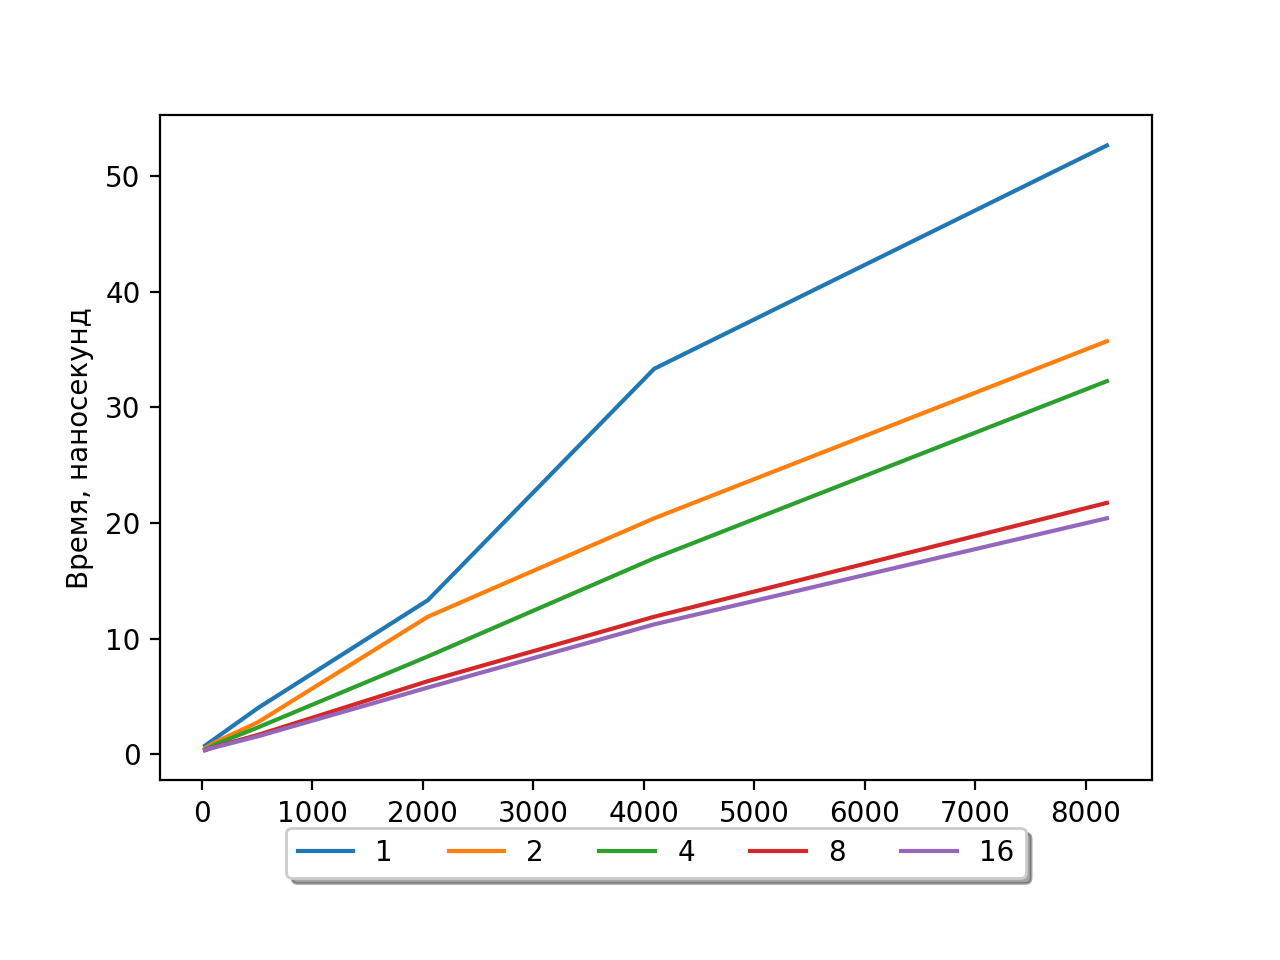
\includegraphics[width=\textwidth]{sem-v-aa-master/lab1/tex/inc/plots/lab4-threads.png}

    \caption{Временные характеристики для различного количества работающих потоков и объектов сцены}
    \label{fig:timestamps}
\end{figure}

\section{Вывод}
В данном разделе было произведено сравнение вышеизложенных алгоритмов.

Наиболее эффективной оказалась параллельная реализация рендеринга, давая прирост производительности более в 2 раза в крайне нагруженной сцене (8192 объекта и их преобразований). Такой прирост был достигнут при использовании 16 потоков.


%%% Local Variables:
%%% mode: latex
%%% TeX-master: "rpz"
%%% End:
